\documentclass[]{article}
\usepackage{amsmath}
\usepackage{verbatim}
\usepackage{array,tabularx}
\usepackage{graphicx}
\graphicspath{ {images/} }
\newenvironment{conditions*}
{\par\vspace{\abovedisplayskip}\noindent
	\tabularx{\columnwidth}{>{$}l<{$} @{\ : } >{\raggedright\arraybackslash}X}}
{\endtabularx\par\vspace{\belowdisplayskip}}
%opening

\title{Understanding urban parking problem with self-driving cars through multiparticle adsorption mechanics}
\author{^We probably need a better title}

\begin{document}

\maketitle

\section*{Introduction}

%%pros and cons of self driving cars
%%surveillance and control
%%congestion impact
%%achievable rate regions

%%notation and setup
%%derivation of denstiy equation


%Self Driving Cars Future has already begun Mr. Muhammad Azmat and Dr. Clemens Schuhmayer
%Institute of Transport and Logistics
%Vienna University Of Economics and Business

%"40 Gasoline is used
%Finding a parking
%spot in Urban Areas"

%"


As self-driving cars become more and more mainstream, we as researchers would like to understand their potential effects on traffic. Numerous benefits of self-driving cars have been recently explored in literature, most notably the ability to go through intersections without stopping \cite{mitSmartIntersect}. One potential benefit of having self-driving cars on the road would be their ability to drop off their passenger and then later on summoned to the spot, essentially eliminating the need for long term parking spots on the road. Even though this is one potential benefit of features like Tesla Summon \cite{teslaSummon}, it is not clear whether this would be beneficial, since cars constantly stopping to pick passengers up and drop them off could cause more congestion. In this paper, we wanted to quantify the effect of such a feature, and to do so, we referred to a well-known stochastic model. 

Totally asymmetric exclusion process (TASEP) has been widely used in various field, ranging from chemistry \cite{chemCoupled} to model vehicular networks \cite{statPhys}. Originated from statistical physics, an instance of TASEP allows deducing macroscopic behavior of the system based upon the microscopic behavior of individual particles. In particular, TASEP is a Markovian process that is defined by the state function and the parameter $p$ such that every particle moves forward with rate $p$ on a one-dimensional lattice. With rate $p$, we refer to the following: every particle has an inner clock that triggers with some constant rate (and thus the time intervals are exponentially distributed and independent) and when the clock of a particle $x$ triggers, $x$ has a chance of $p$ moving forward if the $i+1$th site is empty (thus the exclusion)).   

In this paper, we consider the model developed by Ezaki et al. \cite{adsorption} and improve upon it by including a second-type of particle into the equation which has a different parameter associated with it. This allows us to investigate the potential effects of a second type of car that can avoid congesting a parking spot by dropping its user off. Later in the paper, we extend the model to allow some through traffic and look at achievable rate regions.

%%cite the figure here with the method descriptions

\section*{Model}

For convenience, we repeat the model proposed by Ezaki et al. \cite{adsorption} with slight modifications. 
Let the total number of cars in the ring be a constant $N$.
Every car has an internal timer that triggers with some constant rate (Note: For simulation development, triggering cars with some rate $\omega$ is equivalent to having a global trigger with rate $N\omega$). At any given time, a car $x$ could either be:
\begin{itemize}
\item On the road at a spot $i$ in state A (found parking; trying to get out) or state B(looking for parking) 
\item On the parking lane at a spot $i$ in state C (currently parked).
\end{itemize}

Additionally, every car is either driverless or normal.

Now, when the timer of $x$ goes off, its actions are determined by its state:
\begin{itemize}
	\item State A: If it is a normal car, with probability $\mu_N$, $x$ checks the $i$th spot on the road. If it is empty, it moves there, otherwise, it stays where it is. If it is a driverless car, with probability $\mu_D$, $x$ checks the $i$th spot on the road. If it is empty, it moves there, otherwise, it stays where it is.  
	\item State B: With probability $\lambda$, it check the $i$th parking spot. If it is empty, it moves there, otherwise, it stays where it is.  With probability $p$ (where $\lambda + p \leq 1$), it checks the $i+1$th spot on the road. If it is empty, it moves there, otherwise, it stays where it is.   
	\item State C: With probability $p$, it checks the $i+1$th spot on the road. If it is empty, it moves there, otherwise, it stays where it is.   
\end{itemize}

Before going into analysis, we can define the following notation for clarity:

Normal car refers to a car that is driven by a regular human.

Driverless car (synonymous with self-driving car) refers to a car that does not have a human driver and for this model, is simply a car that does not have to linger as long in a parking spot.

\begin{conditions*}
	A & Car state to denote a car that has parked\\
	B & Car state to denote a car that hasn't parked\\
	C & Car state to denote a car that is parked\\
	S & Element of $\{A,B,C\}$, used to denote one of the states\\ %I don't really use this besides this notation place but oh well
	d  &  Ratio of driverless cars to the total number of cars\\
	L & Total length of the road\\
	N & Total number of cars in the whole system\\
	X & Element of $\{N,D\}$, used to denote one of the car types\\
	i & Element of $\{1,...,L\}$. Used for indexing densities at i th location\\
	\rho_0  &  A constant density \\ % (will be argued for and given an exact form in future sections)
	\rho_i^{tr} & Traffic density at the i th location (i.e. the probability of finding a car on the i th spot on the road on the long run)\\
	\rho _i^S & Density at the i th spot of cars in state S (i.e. the probability of finding a car on the i th spot on the long run, for state A and B, this refers to a spot on the road, for state C, i indexes over the parking spots)\\
	\rho _i^{S_X} & Density of type X cars which are in state S at the i th location\\
	\rho_s & Density of the system ($N/L$)\\
	\lambda & Probability to want to park at the adjacent spot (regardless of the occupancy of the parking spot)\\
	p & Probability to want to move forward (regardless of the occupancy of the next slot)\\
	\mu_X & Probability to want to leave a given spot for a car type X\\
	T_t & Average travel time\\
	T_s & Average time spent in the system\\
	T_a & Average time spent while parked\\
	T_{a_X} & Average time spent while parked for a car of type X\\
\end{conditions*}


%%I'll rewrite the above section; I am aware that from a literary standpoint, repeating the same sentence 15 times is not OK; it just makes my life easier rn.

\section*{Analysis}

%%make a box in illustrator with Brian

Our expression for $\rho_i^{tr}$ stays the same as \cite{adsorption}, and we recite it for convenience:

\begin{align}
\rho_{i-1}^{tr} (1 - \rho_i^{tr}) p = \rho_i^{tr} (1 - \rho_{i+1}^{tr}) p 
\end{align}

\begin{align}
\rho_i^{tr} = \rho_0
\end{align}

These are the balance equations that we will be using to model adding a new type of particle to the system.

\begin{align}
\lambda  \left(1-\rho _i^C\right) \rho _i^{B_N}=\left(1-\rho _0\right)
\mu _N \rho _i^{C_N} \label{eq:Npark}\\
\lambda  \left(1-\rho _i^C\right) \rho
_i^{B_D}=\left(1-\rho _0\right) \mu _D \rho _i^{C_D} \label{eq:Dpark}\\
p \left(1-\rho _0\right)
\rho _{i-1}^{B_N}=\lambda  \left(1-\rho _i^C\right) \rho _i^{B_N}+p
\left(1-\rho _0\right) \rho _i^{B_N} \label{eq:Nroad}\\
p \left(1-\rho _0\right) \rho
_{i-1}^{B_D}=\lambda  \left(1-\rho _i^C\right) \rho _i^{B_D}+p \left(1-\rho
_0\right) \rho _i^{B_D}\label{eq:Droad}\\
\rho _i^{C_D}+\rho _i^{C_N}=\rho _i^C \label{parkingSum}
\end{align}

where \eqref{eq:Npark} is the balance equation for parked normal cars, \eqref{eq:Dpark} is for parked driverless cars, \eqref{eq:Nroad} is for normal cars on road, and \eqref{eq:Droad} is for driverless cars on the road.

When I set $\mu _D = \mu _N$, it agrees with the literature \cite{adsorption}, Eq 7: %%should i put a proof of this in the appendix? 

\begin{align}
\rho _{i-1}^{B_N}\to -\frac{\rho _i^{B_N} \left(\lambda  \left(p \left(\rho _i^{B_D}+\rho _i^{B_N}\right)+\mu _D\right)-p \left(\rho _0-1\right) \mu _D\right)}{p
	\left(\left(\rho _0-1\right) \mu _D-\lambda  \left(\rho _i^{B_D}+\rho _i^{B_N}\right)\right)} \\ \rho _{i-1}^{B_D}\to -\frac{\rho _i^{B_D} \left(\lambda  \left(p \left(\rho
	_i^{B_D}+\rho _i^{B_N}\right)+\mu _D\right)-p \left(\rho _0-1\right) \mu _D\right)}{p \left(\left(\rho _0-1\right) \mu _D-\lambda  \left(\rho _i^{B_D}+\rho
	_i^{B_N}\right)\right)}
\end{align}

Note that both equations are identical, which makes sense, since if these cars were to behave exactly the same, by symmetry, no difference should be observed in their density profiles.

If $\mu _D \not= \mu _N$, then the equations differ, and they become a set of coupled equations.

\begin{align}
\rho _{i-1}^{B_N}\to \frac{\rho _i^{B_N} \left(\lambda  \left(p \mu _N \rho _i^{B_D}+\mu _D \left(p \rho _i^{B_N}+\mu _N\right)\right)-p \left(\rho _0-1\right) \mu
	_D \mu _N\right)}{p \left(\lambda  \mu _N \rho _i^{B_D}+\mu _D \left(\lambda  \rho _i^{B_N}-\rho _0 \mu _N+\mu _N\right)\right)} \label{eq:bn}\\
\rho _{i-1}^{B_D}\to \frac{\rho _i^{B_D}
	\left(\lambda  \left(p \mu _N \rho _i^{B_D}+\mu _D \left(p \rho _i^{B_N}+\mu _N\right)\right)-p \left(\rho _0-1\right) \mu _D \mu _N\right)}{p \left(\lambda  \mu _N \rho
	_i^{B_D}+\mu _D \left(\lambda  \rho _i^{B_N}-\rho _0 \mu _N+\mu _N\right)\right)} \label{eq:bd}
\end{align}

%%is this right??? can i set them to be a constant either way?
Here, we set $\rho^{B_D}_0 = \rho_0 d = \rho_0^D$ and $\rho^{B_N}_0 = \rho_0 (1-d) = \rho_0^N$ as the boundary conditions for this recursive function. Note that we can find the relative densities of $\rho^A$s by subtracting it from the $\rho_0$s, and the density of parking lots from using equations \eqref{eq:Npark} \eqref{eq:Dpark} \eqref{eq:bd} \eqref{eq:bn} and \eqref{parkingSum}.

\subsection*{Parking efficiency}

Now, we can calculate the parking efficiency of the overall system, where we define the concept of the parking efficiency as the ratio of the density of not-parked cars in the L th spot to the total traffic density at that spot of that car type. First, we argue that the parking efficiency of both types of cars are the same. It follows from the observation that given a car enters the system, whether a car parks or not is a function of other cars, and depends on how fast it can get to the parking spot, and whether it will decide to park there or not. Since all those factors are independent from the type of the car, it follows that the parking efficiency is to be the same between these different types of cars. % I think i can mathematically show this as well by arguing q^D = p_0 d - p^{}B_X}_L / p_0 d and the other one and then factor the d s out, but i am not sure whether to do that

In conjunction with this efficiency, we try to find the overall road density $\rho_0$ by following the argument presented in \cite{adsorption}, taking note the crucial part of the argument that the average density $\rho_0/\rho_s$ can be seen as the rate of average occupancy time between the road and the overall system of one car. Since the average time is calculated based upon an expectation, we can further condition this expectation on the type of the car. Thus, we can argue the following equalities:

\begin{align}
\frac{\rho_0}{\rho_s} =& \frac{T_t}{T_s} = \frac{T_t}{T_t + T_a} = \frac{T_t}{T_t + d T_{a_D} + (1 - d) T_{a_N}}\\
	=& \frac{\frac{L}{p (1 - \rho_0)}}{\frac{L}{p (1 - \rho_0)} + d q \frac{1}{\mu_D (1 - \rho_0)} + (1 - d) q \frac{1}{\mu_N (1 - \rho_0)}}
	=& \frac{1}{1 + \frac{pq}{L} (\frac{d}{\mu_d} + \frac{1-d}{\mu_n})}
\end{align}

and since $\rho_s$ is a constant, we can now find $\rho_0$ using this formula.

Now, we try to estimate $q$, and the proof from \cite{adsorption} is identical over here. Note that the approximation from the multiplication of probabilities to sum of their exponentials is expected to be close here, since we expect $\rho_i^C$s to be high in the city setting. Thus, we can reach to a closed form expression for both $\rho_0$ and $q$, and then plot it as follows:

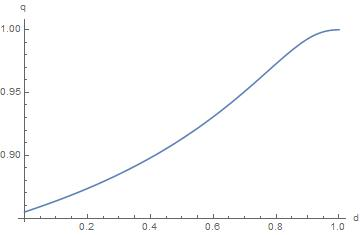
\includegraphics{graph1.jpg}


%graph1.jpg: 
This graph shows how changing the relative ratio of normal cars to driverless cars can affect the parking success rate. For this graph, the following specs were used:
lambda = 0.1;
mun = 0.005;
mud = 0.5;
p = 0.8;
Nt = 20;
L = 30;

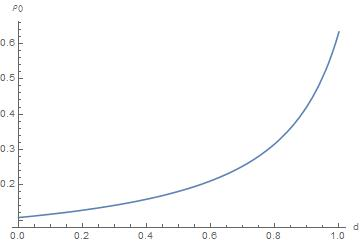
\includegraphics{graph2.jpg}


%graph2.jpg:
 This graph shows how changing the relative ratio of normal cars to driverless cars can affect the road density. For this graph, the following specs were used:
lambda = 0.1;
mun = 0.005;
mud = 0.5;
p = 0.8;
Nt = 20;
L = 30;
\\\\

$\rho_0$ is significant in the sense that $1 - \rho_0$ is directly proportional to the average speed. 


\section*{Extended model}

Next, we extend our model by adding some through traffic. In particular, let the total number of cars still be $N$, but now, divide it into two parts, $N_t$ for people trying to go to town (i.e. park) and $N_v$ for people trying to go to a village (i.e. go through). So, when the timer of a car belonging to $N_t$ group triggers, they don't try to park, they just try to move forward with probability $p$.

If we have everyone trying to go through, this reduces to the known problem of TASEP on a ring, and the solutions for that are explained thoroughly in \cite{statPhys}. Similarly, setting $N_t = 0$ reduces our extended model to our original model.

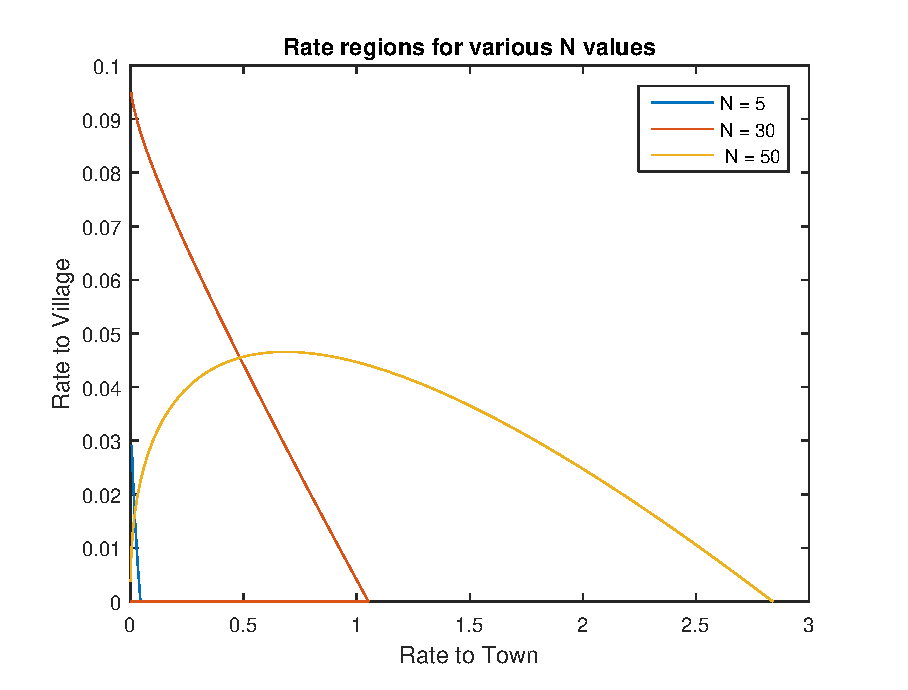
\includegraphics{graph3.eps}

\begin{thebibliography}{9}
\bibitem{nagelGeneric}
STILL FLOWING: APPROACHES TO TRAFFIC FLOW AND
TRAFFIC JAM MODELING

\bibitem{statPhys}	
Statistical physics of vehicular traffic and some related systems

\bibitem{chemCoupled}
Two-channel totally asymmetric simple exclusion
processes

\bibitem{parallelTASEP}
Exact domain wall theory for deterministic TASEP with parallel update

\bibitem{modelPark}
Modeling Parking 

\bibitem{adsorption}
Positive congestion effect on a totally asymmetric simple exclusion process with an adsorption lane

\bibitem{randPark}
The Random Parking Problem 

\bibitem{parkGarage}
Macroscopic car condensation in a parking garage

\bibitem{teslaSummon}
https://www.teslamotors.com/blog/summon-your-tesla-your-phone

\bibitem{mitSmartIntersect}
Revisiting Street Intersections Using SlotBased
Systems
	
\end{thebibliography}



\end{document}
